\documentclass{beamer}
\usetheme{metropolis}

% specifications for presenter mode
%\beamerdefaultoverlayspecification{<+->}
%\setbeamercovered{transparent}

\usepackage[english]{babel}
\usepackage[utf8x]{inputenc}

\usepackage{cancel}
\usepackage{layout}
\usepackage{multirow}
\usepackage{array}
\usepackage{graphicx}
\graphicspath{ {figs/} }

\setbeameroption{hide notes}
\setbeamertemplate{note page}[plain]
\usepackage{listings}
\usepackage{datetime}
\usepackage{url}
\usepackage{tcolorbox}
\usepackage{appendixnumberbeamer}

% math shorthand
\usepackage{bm}
\usepackage{bbm}
\usepackage{amstext}
\usepackage{amsthm}
\usepackage{amsmath}
\usepackage{amsfonts}
\usepackage{amssymb}
\usepackage{mathtools}
\usepackage{mathptmx}
\usepackage{dsfont}
\usepackage{psfrag}
\usepackage{epsfig}
\usepackage{float}
\usepackage{breqn}
\newcommand{\R}{\mathbb{R}}
\newcommand{\D}{\mathcal{D}}
\newcommand{\E}{\mathbb{E}}
\newcommand{\I}{\mathbb{I}}
\newcommand{\pr}{\mathbb{P}}
\newcommand{\F}{\mathcal{F}}
\newcommand{\X}{\mathcal{X}}
\newcommand{\M}{\mathcal{M}}
\newcommand{\lik}{\mathcal{L}}

\newtheorem*{assumption*}{\assumptionnumber}
\providecommand{\assumptionnumber}{}
\makeatletter
\newenvironment{assumption}[2]
 {%
  \renewcommand{\assumptionnumber}{Assumption #1: $\mathcal{#2}$}%
  \begin{assumption*}%
  \protected@edef\@currentlabel{#1: $\mathcal{#2}$}%
 }
 {%
  \end{assumption*}
 }
\makeatother

\DeclarePairedDelimiterX{\infdivx}[2]{(}{)}{%
  #1\;\delimsize\|\;#2%
}
\newcommand{\infdiv}{D\infdivx}
\DeclarePairedDelimiter{\norm}{\lVert}{\rVert}
\DeclareMathOperator*{\argmin}{arg\,min}
\DeclareMathOperator*{\argmax}{arg\,max}

% indepndence notation macro
\newcommand\indep{\protect\mathpalette{\protect\independenT}{\perp}}
\def\independenT#1#2{\mathrel{\rlap{$#1#2$}\mkern2mu{#1#2}}}

% Bibliography
\usepackage{natbib}
\bibpunct{(}{)}{,}{a}{}{;}
\usepackage{bibentry}
% hyperref >= 2026 stubs \hyper@natlinkbreak as {} under beamer's
% implicit=false, eating natbib's author-year space; restore natbib's fallback
\makeatletter
\def\hyper@natlinkbreak#1#2{#1}
\makeatother

%%%%%%%%%%%%%%%%%%%%%%%%%%%%%%%%%%%%%%%%%%%%%%%%%%%%%%%%%%%%%%%%%%%%%%%%%%%%%%%%

% title info
\title{\normalsize Causal machine learning in high-dimensional biology:\\
  Biomarker discovery from biological expression data}
\author{\href{https://nimahejazi.org}{Nima Hejazi}\\[-10pt]}
\institute{
  \begin{figure}[!htb]
    \centering
    \begin{minipage}{.65\textwidth}
        Department of Biostatistics \\
        T.H.~Chan School of Public Health \\
        Harvard University \\[6pt]
        
\includegraphics[scale=0.12]{homepage.png}
          \href{https://nimahejazi.org}{nimahejazi.org} \\
        
\includegraphics[scale=0.09]{github-icon.png}
          \href{https://github.com/nhejazi}{nhejazi} $\vert$
          \href{https://github.com/nshlab}{nshlab} \\
        EMBO course: \underline{Causality in Biomedicine}\\
        European Bioinformatics Institute (EMBL-EBI)\\
        \textit{Joint work with A.~Hubbard, M.~van der Laan, P.~Boileau}
    \end{minipage}%
    \begin{minipage}{0.3\textwidth}
      \centering
      \vspace{-65pt}
      
\includegraphics[width=1.1in]{hsph}
    \end{minipage}
  \end{figure}
}

\date{Wednesday, 7\textsuperscript{th} October 2026}

%%%%%%%%%%%%%%%%%%%%%%%%%%%%%%%%%%%%%%%%%%%%%%%%%%%%%%%%%%%%%%%%%%%%%%%%%%%%%%%%

\begin{document}

\begin{frame}[noframenumbering]
  \thispagestyle{empty}
  \titlepage
\end{frame}

%%%%%%%%%%%%%%%%%%%%%%%%%%%%%%%%%%%%%%%%%%%%%%%%%%%%%%%%%%%%%%%%%%%%%%%%%%%%%%%%

\begin{frame}[c,noframenumbering]{Preview}
\thispagestyle{empty}
\begin{center}
\begin{enumerate}
  \itemsep6pt
  \item Computational biology research produces complex data, but statistical
    methods are often tied to modeling assumptions that are challenging to
    verify from subject matter knowledge.
  \item \textit{Model misspecification} can seriously undermine the scientific
    value of common, parametric statistical modeling approaches.
  \item Semi-parametric inference facilitates construction of robust estimators
    that are compatible with machine learning.
  \item Variance moderation strengthens hypothesis testing strategies, reducing
    false positives and preserving power under instability.
\end{enumerate}
\end{center}

\note{We'll go over this summary again at the end of the talk. Hopefully, it
      will all make more sense then.
}
\end{frame}

%%%%%%%%%%%%%%%%%%%%%%%%%%%%%%%%%%%%%%%%%%%%%%%%%%%%%%%%%%%%%%%%%%%%%%%%%%%%%%%%

\begin{frame}[c]{Sketching a common problem}
\begin{center}
\begin{itemize}
  \itemsep6pt
  \item \textit{Question}: What factors causally impact a health outcome of
    interest (e.g., cancer, death).
  \item \textit{Experiment}: Assign\textsuperscript{?} study units to
    investigational therapy vs.~standard of care and evaluate outcome risk.
  \item \textit{Goal}: Deepen \underline{mechanistic} insights---how does the
    therapy (or exposure) biologically operate? Identify intervention points.
  \item Draw on tools from -omics and molecular biology, clinical trials,
    causal inference, (bio)statistics, epidemiology.
\end{itemize}
\end{center}

\note{
}
\end{frame}

%%%%%%%%%%%%%%%%%%%%%%%%%%%%%%%%%%%%%%%%%%%%%%%%%%%%%%%%%%%%%%%%%%%%%%%%%%%%%%%%

\begin{frame}[c]{Meet the data: Smoking and DNA methylation}
\begin{center}
\begin{itemize}
  \itemsep6pt
  \item \textit{Question}: Which CpG sites, or larger functional units (e.g.,
    CpG islands) are affected by long-term smoking?
  \item \textit{Why?} Attempt to understand how smoking induces regulatory and
    functional changes that relate to disease (e.g., cancer).
  \item \textit{Study}: Observational exposure study of $253$ individuals (172
    smokers, 81 non-smokers) with 450,000 CpG sites assayed.
  \item \textit{Goal}: Characterize biological mechanisms, signatures, or
    biomarkers derived from or attributable to smoking.
\end{itemize}
\end{center}

\note{
}
\end{frame}

%%%%%%%%%%%%%%%%%%%%%%%%%%%%%%%%%%%%%%%%%%%%%%%%%%%%%%%%%%%%%%%%%%%%%%%%%%%%%%%%

\begin{frame}[c]{Data structure and notation}
\begin{center}
\begin{itemize}
  \itemsep6pt
  \item Consider a structural causal model~\citep{pearl2000causality} that
    describes the data-generating process for a single unit $O$:
    \begin{equation*}\label{npsem}
        L = f_L(U_L); A = f_A(L, U_A); Y = f_Y(A, L, U_Y).
      \end{equation*}
  \item $f_L$, $f_A$, $f_Y$ are unknown, deterministic functions; $U_L$, $U_A$,
    $U_Y$ are exogenous, unobserved errors, assumed $U_L \indep U_A \indep
    U_Y$.
  \item $Y = (Y_b: b = 1, \ldots, B)$ is a vector of biomarker outcomes, where
    we have, e.g., $B = 450,000$ CpG sites.
  \item Temporal ordering between variables: $L$ (sex-at-birth, age), $A$
    (smoking), $Y_b$ (outcome at CpG site $b$).
  \item Data on a single study unit $O = (L, A, Y)$, with $O \sim \mathsf{P}_0
    \in \mathcal{P}$, of which we observe $n$ i.i.d.~copies, $O_1, \ldots,
    O_n$.
\end{itemize}
\end{center}

\note{
}
\end{frame}

%%%%%%%%%%%%%%%%%%%%%%%%%%%%%%%%%%%%%%%%%%%%%%%%%%%%%%%%%%%%%%%%%%%%%%%%%%%%%%%%

\begin{frame}[c]{Hypothetical interventions and causal inference}
\begin{center}
\begin{itemize}
  \itemsep6pt
  \item \textit{Static} interventions consider replacing $f_A$ with an assigned
    value $a \in \mathcal{A}$ deterministically: ``What if everyone smoked?''
  \item Generates counterfactual RV $Y(a) = (Y_b(a), b = 1, \ldots, B)$: the
    expression of the $B$ biomarkers if $A$ had been set to $a$.
  \item Viewed as \textit{potential outcomes} (POs)~\citep{rubin2005causal},
    $Y_b(1)$ when setting $A=1$ and $Y_b(0)$ when setting $A = 0$.
  \item Note $Y_b = A Y_b(1) + (1 - A) Y_b(0)$, this partial visibility is the
    \textit{fundamental problem of causal
    inference}~\citep{holland1986statistics}.
  \item Causal inference yields interpretable, scientifically well-aligned
    estimands, e.g., the average treatment effect (ATE).
\end{itemize}
\end{center}

\note{Statistical parameter may be viewed as a simple adjusted difference in
  means even when identifiability conditions may not be satisfied.
}
\end{frame}

%%%%%%%%%%%%%%%%%%%%%%%%%%%%%%%%%%%%%%%%%%%%%%%%%%%%%%%%%%%%%%%%%%%%%%%%%%%%%%%%


\begin{frame}[c]{A familiar workhorse: the linear model}
\begin{center}
\begin{itemize}
  \itemsep6pt
  \item The linear model is \textit{flexible}? Linear in parameters!
  \item Flexibility: transformations ($X_j^2$), interactions ($X_j X_k$).
  \item For biomarker $Y_b$, fit \textit{working} linear model,
    $\mathbb{E}_0[Y_b \mid \mathbf{X}] = \mathbf{X} \beta$; if $X_1 \equiv A$
      is the exposure, then $\beta_1$ measures its impact on $Y$.
  \item Under this working model, $\beta_1$ is a \textit{conditional} effect
    measure, whose interpretation depends on $\mathbf{X} \setminus X_1$, and
    which coincides with the ATE only under randomization.
  \item Test the contrast of interest with a standard t-test:
    $$ t_{b} = \frac{\hat{\beta}_{b} - \beta_{b, H_0}}{\hat{\sigma}_b} $$
\end{itemize}
\end{center}

\note{There's nothing particularly wrong with this approach. It's exactly what
      we would come up with after a first-year statistics course. In practice,
      there are many issues: (1) we are forced to specify a functional form, the
      linear model; (2) we end up with unstable variance estimates that sharply
      increase the number of false positives detected, even after multiple
      testing corrections. In practice, the incredible flexibility of the linear
      mode is rarely taken advantage of---scientific guidance is usually
      lacking to justify fitting richer models.
}
\end{frame}

%%%%%%%%%%%%%%%%%%%%%%%%%%%%%%%%%%%%%%%%%%%%%%%%%%%%%%%%%%%%%%%%%%%%%%%%%%%%%%%%

\begin{frame}[c]{Variance moderation to the rescue?!}

\begin{center}
\begin{itemize}
  \itemsep6pt
  \item When sample size is small, $\hat{\sigma}^2_b$ may be so small (by
    chance) that even small effect sizes ($\hat{\beta}_{b} - \beta_{b, H_0}$)
    yield large $t_b$.
  \item False positives! Many biomarkers flagged relevant despite small effect
    size, only since variance is even smaller still.
  \item Can we do better? A \textbf{moderated} t-test~\citep{smyth2004linear}:
    $$
      \tilde{t}_{b} = \frac{\hat{\beta}_{b} - \beta_{b, H_0}}{\tilde{\sigma}_b}
      \quad \text{where} \quad
      \tilde{\sigma}^2_b = \frac{\hat{\sigma}^2_b d_b + \hat{\sigma}^2_0
        d_0}{d_b + d_0}
    $$
  \item Helps reduce erroneously large $t_b$ by ``averaging out'' low variance
    across each of the many biomarkers.
\end{itemize}
\end{center}

\note{The substantive contribution here is the use of an empirical Bayes method
      to shrink the standard deviation across all the biomarkers such that we
      obtain a larger (but accurate) estimate that reduces the number of test
      statistics that are marked as significant by low $s^2_b$ estimates alone.

      Note that this is \textbf{not} the exact formulation of the moderated
      t-statistic as given by Smyth (his derivation assumes a hierarchical
      model; see original paper if interested). This formulation does a good
      enough job to help us see the bigger picture.
}
\end{frame}

%%%%%%%%%%%%%%%%%%%%%%%%%%%%%%%%%%%%%%%%%%%%%%%%%%%%%%%%%%%%%%%%%%%%%%%%%%%%%%%%

\begin{frame}[c]{Variable importance measures as target parameters}

\begin{center}
\begin{itemize}
  \itemsep6pt
  %\item If the working model is incorrect, $\beta_b$ does not correspond to the
    %ATE $\theta^{\text{ATE}}$ --- \textit{identification bias}.
  \item The statistical functional identifying the ATE ($\psi_{b,0}$) may be
    used as an estimand to assess variable importance:
    \begin{align*}
      \theta^{\text{ATE}} &= \mathbb{E}[Y_b(1) - Y_b(0)] \\
      \psi_{b,0} \coloneqq \Psi_b(\mathsf{P}_0) &=
        \mathbb{E}_{L,0}\{\mathbb{E}_0[Y_b \mid A = 1, L] -
        \mathbb{E}_0[Y_b \mid A = 0, L]\}
    \end{align*}
  \item $\psi_{b,0}$ is a mapping, $\Psi_b(\mathsf{P}_0)$, that depends on the
    underlying true (but unknown) distribution $\mathsf{P}_0 \in \mathcal{P}$
    (model-agnostic!)
  \item The causal parameter $\theta^{\text{ATE}}$ is identified by the
    statistical functional $\psi_{b,0}$ under some assumptions (no unmeasured
    confounding, positivity), i.e., $\theta^{\text{ATE}} \equiv \psi_{b,0}$.
\end{itemize}
\end{center}

\note{By allowing scientific questions to inform the parameters that we choose
      to estimate, we can do a better job of actually answering the questions of
      interest to our collaborators. Further, we abandon the need to specify the
      functional relationship between our outcome and covariates; moreover, we
      can now make use of advances in machine learning.
}
\end{frame}

%%%%%%%%%%%%%%%%%%%%%%%%%%%%%%%%%%%%%%%%%%%%%%%%%%%%%%%%%%%%%%%%%%%%%%%%%%%%%%%%

\begin{frame}[c]{Locally efficient estimation}

\begin{center}
\begin{itemize}
  \itemsep6pt
  \item An estimator $\hat{\psi}_b$ is \textit{asymptotically linear} if it
    admits the form
    $$ \sqrt{n}(\hat{\psi}_b - \psi_{b,0}) = \frac{1}{\sqrt{n}}
      \sum_{i = 1}^{n} D_b(O_i; \mathsf{P}_0) + o_{\mathsf{P}}(1) \ , $$
      where $D_b(O; P_0)$ is the efficient influence function (wrt
      $\mathcal{P}$), whose asymptotic variance at $\mathsf{P}_0$ is the
      \textit{efficiency bound}.
  \item $D_b(O; \mathsf{P}_0)$ helpful to construct efficient estimators. For
    ATE,
    \begin{align*}
      D_b (O_i; \mathsf{P}_0) =& \left(\frac{2A_i - 1}{g_0(L_i)} \right)
      [Y_{b, i} - \overline{Q}_{0,b}(A_i, L_i)] + \\ 
      &[\overline{Q}_{0,b}(1, L_i) - \overline{Q}_{0,b}(0, L_i)] -
      \psi_{b, 0} \ ,
    \end{align*}
    where $g_0(L) = \mathbb{P}_0(A = 1 \mid L)$ is the propensity score
    and $\overline{Q}_{0,b}(A,L) = \mathbb{E}_0[Y_b \mid A, L]$ the conditional
    outcome mean.
\end{itemize}
\end{center}

\note{Natural use of machine learning methods for the estimation of both $Q_0$
      and $g_0$. Focuses effort to achieve minimal bias and asymptotic
      semi-parametric efficiency bound for the variance, but still get
      inference (with some assumptions).
}
\end{frame}

%%%%%%%%%%%%%%%%%%%%%%%%%%%%%%%%%%%%%%%%%%%%%%%%%%%%%%%%%%%%%%%%%%%%%%%%%%%%%%%%

\begin{frame}[c]{Constructing locally efficient estimators}

\begin{center}
\begin{itemize}
  \itemsep6pt
  \item Examining $D_b(O; \mathsf{P}_0)$, we know we must estimate $g_0(L)$ and
    $\overline{Q}_{0,b}(A,L)$, but how to do this?
  \item No need to try to exactly specify functional forms or assume we know the
    underlying true data-generating distribution $\mathsf{P}_0$.
  \item Machine learning of $g_0(L)$ and $\overline{Q}_{0,b}(A,L)$, e.g., by
    ensembling, stacking~\citep{vdl2007super, breiman1996stacked}.
  \item One-step estimator~\citep{bickel1993efficient} uses ``debiasing'' based
    on an additive correction:
    $\hat{\psi}_{b}^{+} = \hat{\psi}_{b}^{\text{PI}} +
    n^{-1} \sum_{i=1}^n \hat{D}_b(O_i)$.
  \item A valid variance estimator: $\hat{\mathbb{V}}(\hat{\psi}_b^{+}) =
    n^{-1} \sum_{i=1}^n \hat{D}_b^2(O_i)$, but its small-sample behavior may be
    erratic (asymptotically valid).
\end{itemize}
\end{center}

\note{Natural use of machine learning methods for the estimation of both $Q_0$
      and $g_0$. Focuses effort to achieve minimal bias and asymptotic
      semi-parametric efficiency bound for the variance, but still get
      inference (with some assumptions).
}
\end{frame}

%%%%%%%%%%%%%%%%%%%%%%%%%%%%%%%%%%%%%%%%%%%%%%%%%%%%%%%%%%%%%%%%%%%%%%%%%%%%%%%%

\begin{frame}[c]{Moderated test statistics with efficient influence functions}

\begin{center}
\begin{itemize}
  \itemsep6pt
  \item Moderated t-statistic of~\cite{smyth2004linear} can be paired with
    locally efficient estimators:
    \begin{equation*}
      \tilde{t}_b = \frac{\hat{\psi}_b^{+} - \cancel{\psi_{b,0}}{~^{
      \scriptstyle H_0:~\psi_{b,0} = 0}}}
      {\tilde{\sigma}_b},
    \end{equation*}
    where the \textit{moderated} (influence function) variance is
    \begin{equation*}
      \tilde{\sigma}^2_b = \frac{\hat{\sigma}^2_b d_b + \hat{\sigma}^2_0 d_0}
      {d_b + d_0}
    \end{equation*}
  \item Preserves robust variance estimator while adding stability by
    ``averaging out'' potentially erratic variance across biomarkers.
  \item Avoid model misspecification while stabilizing inference.
\end{itemize}
\end{center}

\note{
}
\end{frame}

%%%%%%%%%%%%%%%%%%%%%%%%%%%%%%%%%%%%%%%%%%%%%%%%%%%%%%%%%%%%%%%%%%%%%%%%%%%%%%%%

\begin{frame}[c,noframenumbering,plain]{Numerical study: Rare effect (10\%)
without positivity issues}

\centering
\includegraphics[origin=c,scale=0.205]{fdr_sl_findings_min_logistic_g0prob_no}

\note{
Setting: strong exposure effect in 10\% of biomarkers and no positivity issues
in the exposure mechanism.
}
\end{frame}

%%%%%%%%%%%%%%%%%%%%%%%%%%%%%%%%%%%%%%%%%%%%%%%%%%%%%%%%%%%%%%%%%%%%%%%%%%%%%%%%

\begin{frame}[c,noframenumbering,plain]{Numerical study: Common effect (30\%)
with positivity issues}

\centering
\includegraphics[origin=c,scale=0.205]{fdr_sl_findings_mod_logistic_g0prob_yes}

\note{
Setting: strong exposure effect in 30\% of biomarkers and notable positivity
issues in the exposure mechanism.
}
\end{frame}

%%%%%%%%%%%%%%%%%%%%%%%%%%%%%%%%%%%%%%%%%%%%%%%%%%%%%%%%%%%%%%%%%%%%%%%%%%%%%%%%

\begin{frame}[c]{Differential expression analysis procedure}

\begin{center}
\begin{enumerate}
  \itemsep6pt
  \item Apply a filtering procedure to reduce the set of candidate
    biomarkers~\citep{tuglus2009modified} \textit{optionally}.
   \item For each biomarker, generate an efficient estimate $\hat{\psi}_b$ of
    $\psi_{0,b}$ with EIF $\hat{D}_b(O_i)$ after estimating nuisances $(g_0,
    \overline{Q}_{0,b})$.
  \item Apply variance moderation across the EIF estimates, yielding
    \textit{moderated} $\tilde{\sigma}_b^2$, to be used for stabilized
    hypothesis testing.
  \item Hypothesis testing from moderated test statistics can be made
    ``optimistic'' (MVN) or conservative (logistic).
  \item Apply a multiple testing correction for accurate simultaneous inference
    across all $B$ biomarkers, e.g., by controlling the False
    Discovery Rate~\citep{benjamini1995controlling}.
\end{enumerate}
\end{center}

\note{
}
\end{frame}

%%%%%%%%%%%%%%%%%%%%%%%%%%%%%%%%%%%%%%%%%%%%%%%%%%%%%%%%%%%%%%%%%%%%%%%%%%%%%%%%

\begin{frame}[c]{Applying the differential expression procedure}

\begin{center}
\begin{enumerate}
  \itemsep6pt
  \item Filtered set of 450,000 CpG sites measured down to 2537 CpG sites by
    covariate adjustment in a working linear model.
   \item For each candidate CpG (among 2537), estimate $(g_0,
     \overline{Q}_{0,b})$ by super (ensemble) learning, then construct efficient
     estimate $\hat{\psi}_b$ of ATE from the EIF $\hat{D}_b(g_n,
     \overline{Q}_{n,b})$.
  \item Variance moderation based on estimated EIF, yielding \textit{moderated}
    $\tilde{\sigma}_b^2$, for stabilized hypothesis testing across CpGs.
  \item Applied Holm's procedure to control the family-wise error rate (FWER),
    tagging 1173 CpG sites as differentially methylated.
  \item Top CpG site (cg05575921) lies in the AHRR gene, previously
    identified in at least 30 epigenome-wide association studies on impact of
    smoking exposure on blood and lung tissues.
\end{enumerate}
\end{center}

\note{
}
\end{frame}

%%%%%%%%%%%%%%%%%%%%%%%%%%%%%%%%%%%%%%%%%%%%%%%%%%%%%%%%%%%%%%%%%%%%%%%%%%%%%%%%

\begin{frame}[c,noframenumbering,plain]{Ranking differentially methylated CpGs}

\centering
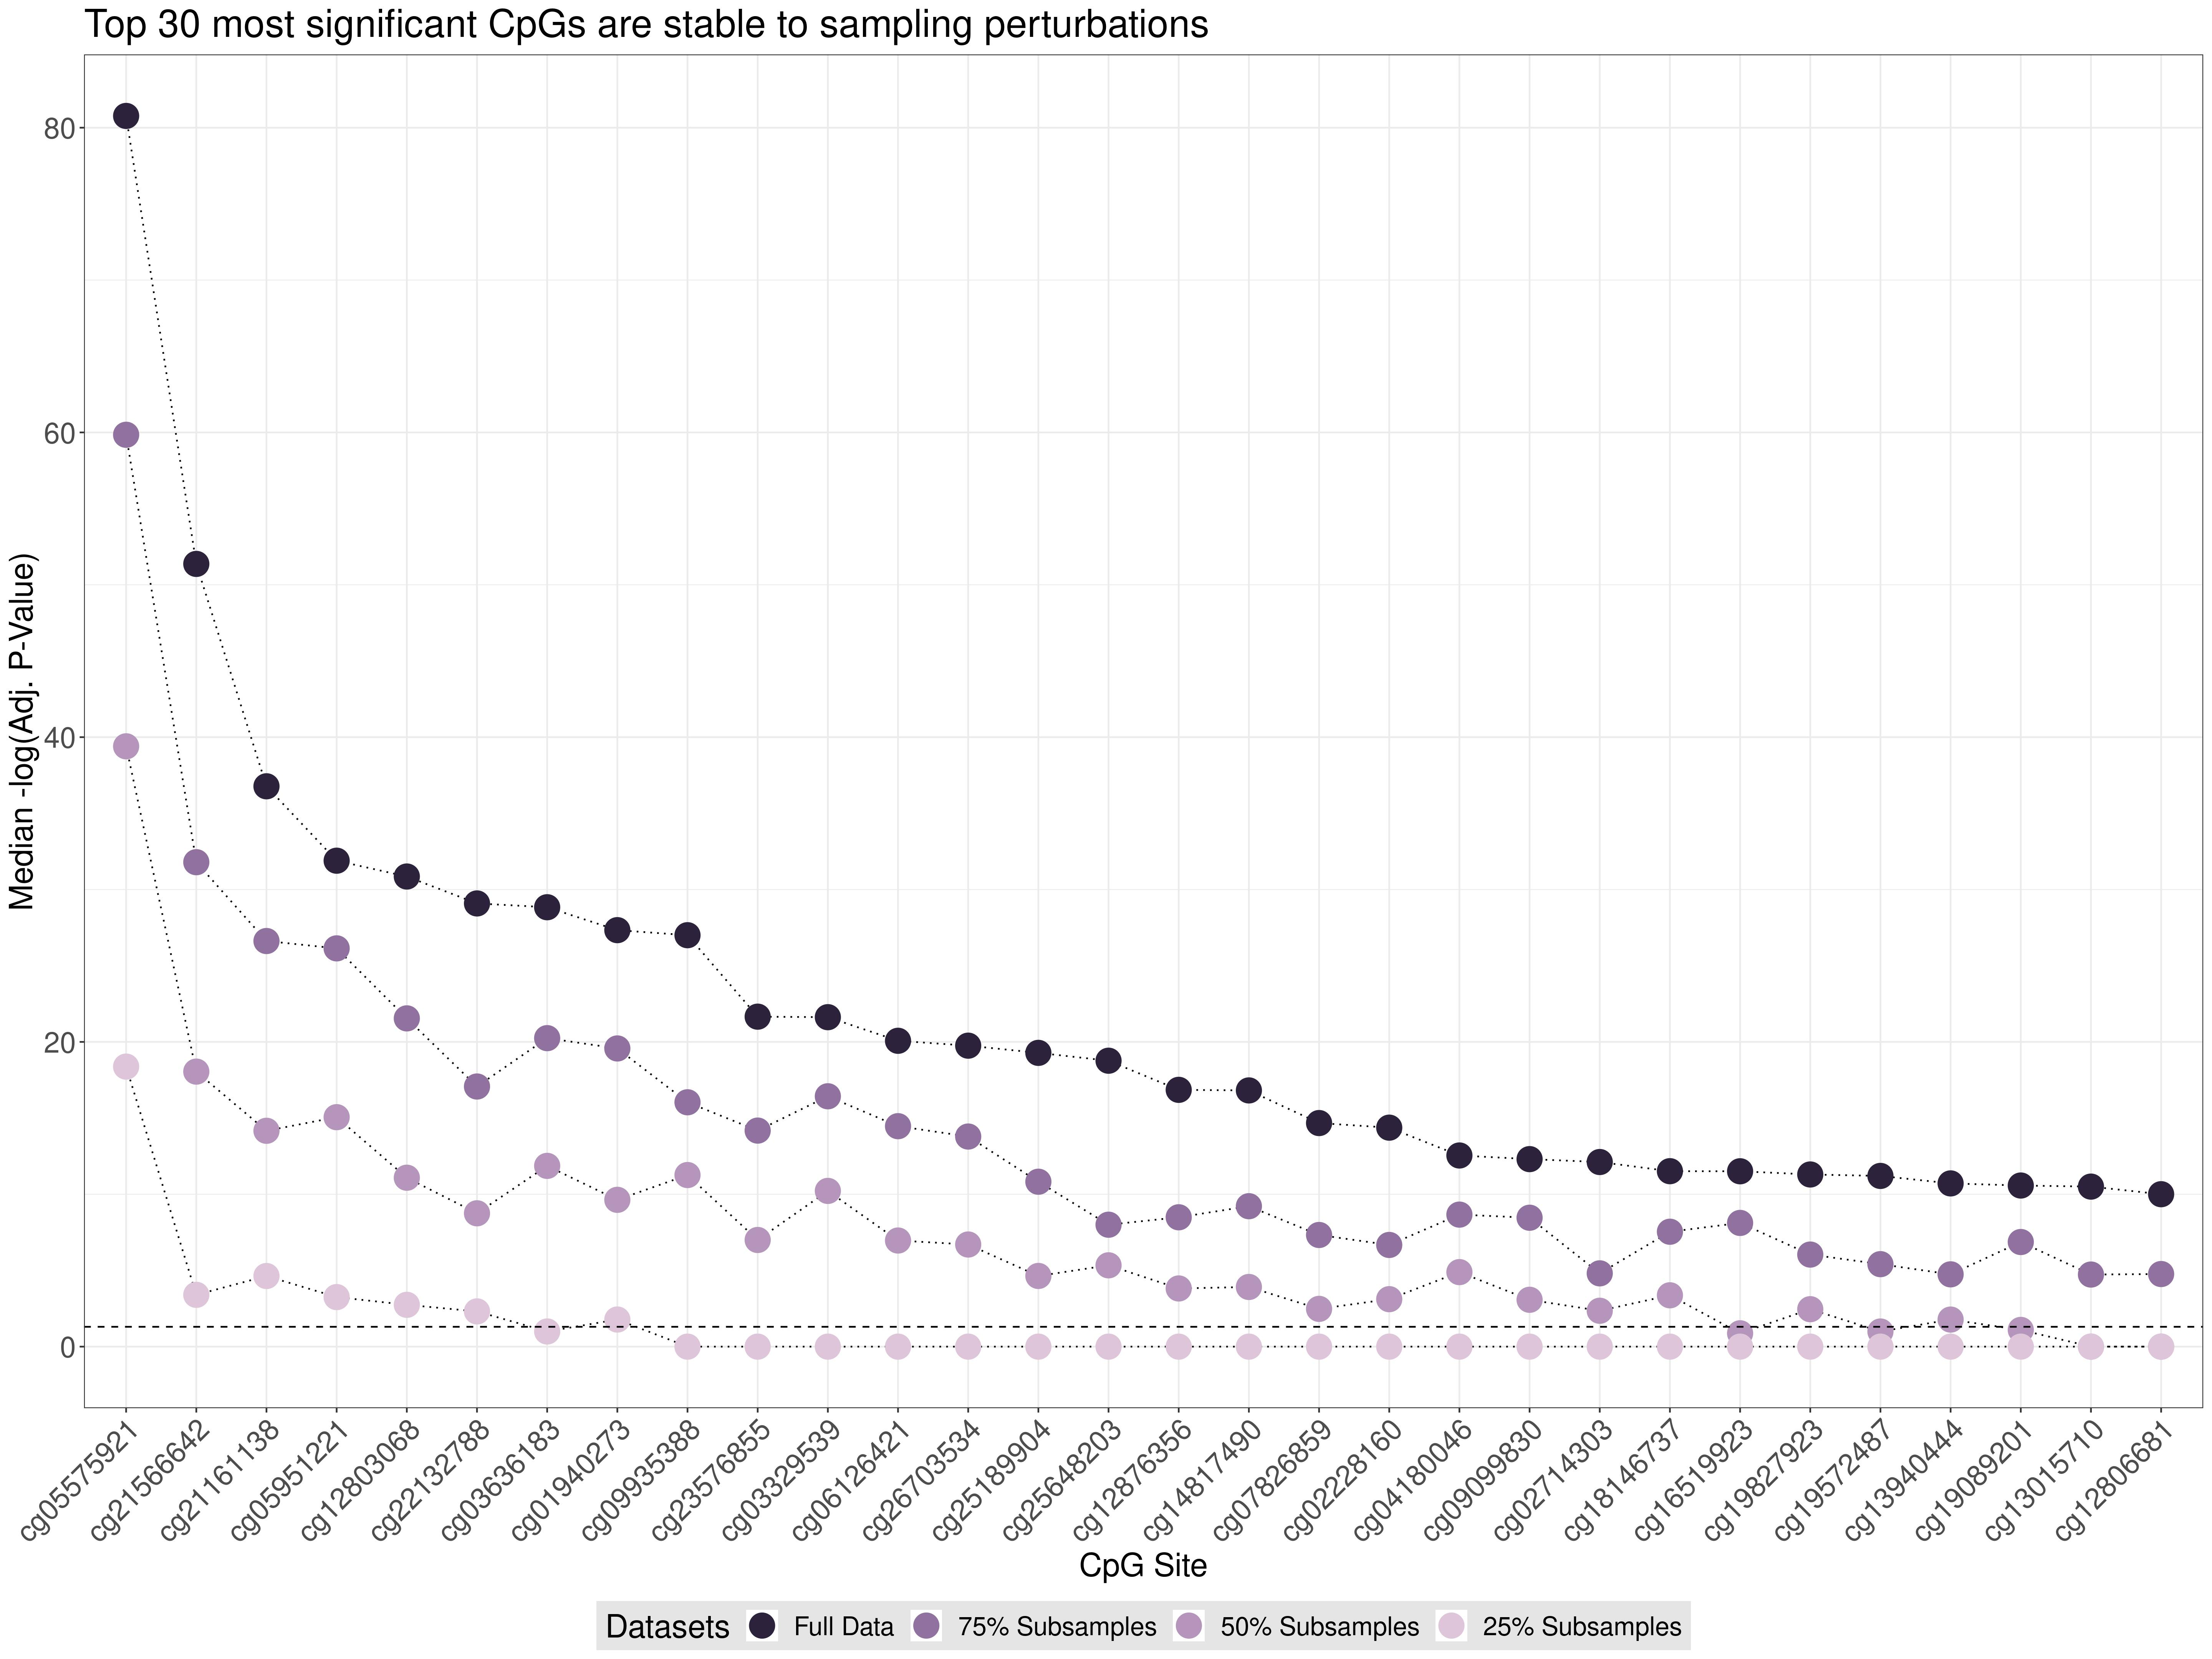
\includegraphics[origin=c,scale=0.22]{cpg_ranks}

\note{
}
\end{frame}

%%%%%%%%%%%%%%%%%%%%%%%%%%%%%%%%%%%%%%%%%%%%%%%%%%%%%%%%%%%%%%%%%%%%%%%%%%%%%%%%

\begin{frame}[c]{Open-source software: \texttt{R/biotmle}}

\begin{center}
\begin{itemize}
  \itemsep6pt
  \item \texttt{R} package for differential expression or methylation analysis
     based on \textit{model-agnostic}, efficient estimators of the ATE.
  \item Incorporates machine learning and allows cross-validation.
  \item Statistical inference based on semi-parametric efficiency theory
    \textit{and} variance moderation.
  \item Where can you find it?
    \begin{itemize}
      \itemsep4pt
      \item \url{https://github.com/nhejazi/biotmle}
      \item \url{https://bioconductor.org/packages/biotmle}
    \end{itemize}
\end{itemize}
\end{center}

\note{Use it. File an issue. Help make it better!
}
\end{frame}

%%%%%%%%%%%%%%%%%%%%%%%%%%%%%%%%%%%%%%%%%%%%%%%%%%%%%%%%%%%%%%%%%%%%%%%%%%%%%%%%

\begin{frame}[c,noframenumbering]{Review}
\thispagestyle{empty}
\begin{center}
\begin{enumerate}
  \itemsep6pt
  \item Computational biology research produces complex data, but statistical
    methods are often tied to modeling assumptions that are challenging to
    verify from subject matter knowledge.
  \item \textit{Model misspecification} can seriously undermine the scientific
    value of common, parametric statistical modeling approaches.
  \item Semi-parametric inference facilitates construction of robust estimators
    that are compatible with machine learning.
  \item Variance moderation strengthens hypothesis testing strategies, reducing
    false positives and preserving power under instability.
\end{enumerate}
\end{center}

\note{It's always good to include a summary.}
\end{frame}

%%%%%%%%%%%%%%%%%%%%%%%%%%%%%%%%%%%%%%%%%%%%%%%%%%%%%%%%%%%%%%%%%%%%%%%%%%%%%%%%

% don't want dimming with references
\setbeamercovered{}
\beamerdefaultoverlayspecification{}

\begin{frame}[c,allowframebreaks]{}

\small
\bibliographystyle{apalike}
%\nocite{*}
\bibliography{references}

\end{frame}

%%%%%%%%%%%%%%%%%%%%%%%%%%%%%%%%%%%%%%%%%%%%%%%%%%%%%%%%%%%%%%%%%%%%%%%%%%%%%%%%

\begin{frame}[c]{Thank you! Questions?}


\includegraphics[scale=0.14]{homepage.png} \url{https://nimahejazi.org}

\vspace{2mm}

\includegraphics[scale=0.11]{github-icon.png}
  \url{https://github.com/nshlab}

\vspace{2mm}

\includegraphics[scale=0.11]{github-icon.png}
  \url{https://github.com/nhejazi}

\vspace{2mm}

\includegraphics[scale=0.14]{pdf-icon.png}
  \url{https://doi.org/10.1177/09622802221146313}

\note{Here's where you can find me, as well as the slides for this talk.}

\end{frame}

\end{document}
